\documentclass[12pt]{report}

\usepackage[utf8]{inputenc}
\usepackage{graphicx}
\usepackage{amsmath,amssymb}
\usepackage{fancyhdr}
\usepackage{setspace}
\usepackage{longtable}
\usepackage{caption}
\usepackage[margin=1in]{geometry}
\usepackage{titlesec}
\usepackage{changes}
\usepackage{color,soul}
\usepackage{subcaption}
\usepackage{tabularx}
\usepackage{booktabs}
\usepackage{multirow}
\usepackage[authoryear]{natbib}           % choose [numbers] or [authoryear]
\usepackage[acronym]{glossaries}
\makeglossaries                             % REQUIRED for \printglossary (indexed)
\usepackage{array,xcolor,colortbl}
\usepackage{tikz}
\usetikzlibrary{shapes.geometric, arrows.meta, positioning}

\definecolor{morange}{rgb}{0.8,0.2,0}
\definecolor{mblue}{rgb}{0,0.1,0.8}
\definecolor{mgreen}{rgb}{0,0.8,0.1}
\definecolor{mred}{rgb}{1,0,0}

\setglossarystyle{long}
\newcommand{\edit}[1]{{\leavevmode\color{mblue}{#1}}}
\newcommand{\kais}[1]{{\color{morange}{{(\bf Kais:} #1)}}}

\titleformat{\chapter}[hang]{\bfseries\Large}{Chapter \thechapter}{2em}{}
\onehalfspacing

\pagestyle{fancy}
\fancyhf{}
\fancyfoot[C]{\thepage}

%\input{Thesis_proposal/acronyms/acronyms}

\usepackage[hidelinks]{hyperref}          % LOAD HYPERREF LAST

%==============================================================


%\titleformat{\chapter}[hang]{\bfseries\Large}{Chapter \thechapter}{2em}{}

%\onehalfspacing

% Header/Footer setup
%\pagestyle{fancy}
%\fancyhf{}
% Acronym definitions for Driver Monitoring System Project

% DMS Primary Acronyms
\newacronym{dms}{DMS}{Driver Monitoring System}
\newacronym{ir}{IR}{Infrared}
\newacronym{rgb}{RGB}{Red-Green-Blue}
\newacronym{uae}{UAE}{United Arab Emirates}
\newacronym{eu}{EU}{European Union}
\newacronym{gsr}{GSR}{General Safety Regulation}
\newacronym{yolo}{YOLO}{You Only Look Once}
\newacronym{coco}{COCO}{Common Objects in Context}
\newacronym{fps}{FPS}{Frames Per Second}
\newacronym{tls}{TLS}{Transport Layer Security}
\newacronym{gps}{GPS}{Global Positioning System}
\newacronym{roi}{ROI}{Region of Interest}
\newacronym{rta}{RTA}{Roads and Transport Authority}
\newacronym{sdp}{SDP}{Senior Design Project}
\newacronym{ema}{EMA}{Exponential Moving Average}
\newacronym{led}{LED}{Light Emitting Diode}
\newacronym{usb}{USB}{Universal Serial Bus}
\newacronym{flop}{FLOP}{Floating Point Operation}
\newacronym{ear}{EAR}{Eye Aspect Ratio}
\newacronym{perclos}{PERCLOS}{Percentage of Eye Closure}
\newacronym{wal}{WAL}{Write-Ahead Logging}
\newacronym{ui}{UI}{User Interface}
\newacronym{ux}{UX}{User Experience}
\newacronym{poi}{POI}{Point of Interest}
\newacronym{fp}{FP}{False Positive}
\newacronym{ac}{AC}{Air Conditioning}
\newacronym{npu}{NPU}{Neural Processing Unit}
\newacronym{api}{API}{Application Programming Interface}
\newacronym{ipc}{IPC}{Inter-Process Communication}

% Legacy / Secondary references
\newacronym{uav}{UAV}{Unmanned Aerial Vehicle}
\newacronym{mitm}{MitM}{Man-in-the-Middle}
\newacronym{abe}{ABE}{Attribute-Based Encryption}
\newacronym{faa}{FAA}{Federal Aviation Administration}
\newacronym{sora}{SORA}{Specific Operations Risk Assessment}
\newacronym{fmea}{FMEA}{Failure Mode and Effects Analysis}
\newacronym{stpa}{STPA}{Systems-Theoretic Process Analysis}
\newacronym{eta}{ETA}{Event Tree Analysis}
\newacronym{fta}{FTA}{Fault Tree Analysis}
\newacronym{bn}{BN}{Bayesian Network}
\newacronym{cagr}{CAGR}{Compound Annual Growth Rate}
\newacronym{usa}{USA}{United States of America}
\newacronym{uk}{UK}{United Kingdom}
\newacronym{jarus}{JARUS}{Joint Authorities for Rulemaking on Unmanned Systems}
\newacronym{utm}{UTM}{Unmanned Aircraft System Traffic Management}
\newacronym{rid}{RID}{Remote identification}
\newacronym{easa}{EASA}{European Union Aviation Safety Agency}
\newacronym{icao}{ICAO}{International Civil Aviation Organization}
\newacronym{d3s}{D3S}{Drone Security Scoring System}
\newacronym{oso}{OSO}{Operational Safety Objectives}
\newacronym{caa}{CAA}{Civil Aviation Authority}
\newacronym{mit}{MIT}{Massachusetts Institute of Technology}
\newacronym{adasi}{ADASI}{Advanced Military Systems \& Solutions}
\newacronym{isr}{ISR}{Intelligence, Surveillance, and Reconnaissance}
\newacronym{gcaa}{GCAA}{General Civil Aviation Authority}
\newacronym{rf}{RF}{Radio Frequency}
\newacronym{c-uas}{C-UAS}{Counter-Unmanned Aircraft System}
\newacronym{crs}{CRS}{Composite Risk Score}


% Begin document
\begin{document}

% Title Page
\begin{titlepage}
    \centering
    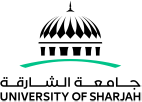
\includegraphics[width=0.25\textwidth]{Figures/Logo_UoS.png}

    \textsc{\Large College of Computing and Informatics\\
    Department of Computer Engineering}\\[1.5cm]
    
    \textsc{\Large SDP Proposal}\\[0.5cm]
    
    \rule{\linewidth}{0.5mm} \\[0.4cm]
    {\LARGE \bfseries Design and Implementation of an Edge-Based Driver Monitoring System with False Alarm Reduction}\\[0.4cm]
    \rule{\linewidth}{0.5mm} \\[1.5cm]
    
    \begin{flushleft}
    \textbf{Students:} \\
    Oumar Mamoun Ibrahim (U22200741) \\
    Abdullah Jafar Abdelhamid (U23101327) \\
    Faris Munadhil Ahmed Alagha (U23104246) \\
    Mohamed Ahmed Saad Khafagy (U20101649) \\[0.3cm]
    \textbf{Supervisor:} Dr. Mohamad Khairi Bin Ishak \\
    \textbf{Term:} Fall 2026--2027
    \end{flushleft}

    \vfill

     \textbf{Date:} \today
    \vspace*{1cm}
       
\end{titlepage}

% Table of Contents, List of Figures, Tables
\tableofcontents

\newpage


\listoffigures
\listoftables
\newpage
\printglossary[type=\acronymtype, title=Acronyms]
\newpage

% Abstract
\chapter*{Abstract}
\addcontentsline{toc}{chapter}{Abstract}
In-cabin Driver Monitoring Systems (DMS) play an increasingly vital role in road safety, particularly as regulatory bodies such as the European Union (GSR 2024) mandate automated alertness and distraction detection in all newly registered vehicles. However, conventional commercial and edge-deployed systems suffer from elevated false alarm rates, triggering nuisance alerts that induce driver frustration, cognitive fatigue, and system deactivation. This Senior Design Project presents a reliable, edge-based Driver Monitoring System deployed on the Raspberry Pi 5 platform paired with a 1080p 30 FPS RGB camera. The architecture integrates a fine-tuned YOLO11n object detector with hard-negative mining, casual exponential moving average (EMA) temporal filtering, mirror-check suppression, camera-blindness detection, and tiered multi-modal alerts in English and Arabic. Furthermore, privacy-preserving event logging with power-cut-safe SQLite WAL storage synchronizes with an interactive desktop and tablet dashboard providing behavioral trends, safety KPIs, and intelligent rest-stop suggestions.


\chapter{Introduction}
\section{Problem Statement and Proposed Solution}

\glspl{dms} evolved since they got introduced in 2006 \cite{r7}. Transitioning from merely alerting the driver through an \gls{ir} camera and applying breaks \cite{r8}, to tracking eye gaze and fusing it with vehicular spatial awareness \cite{r9}. Conversely, nuisance alerts and false alarms causes driver distrust in these systems, causing system neglect or circumvention \cite{r10}. The gap falls under improving the user experience in theses systems. Given the \gls{uae} context of high speed highways, and the need for private and trustworthy systems. We aim to deliver a system that is built the supplement the driver's attention and not replace it. Figure \ref{fig:1.1} shows the results of in-attentive driving, which stresses the need for these systems to be deployed at a greater rate. In 2024, \gls{eu}’s \gls{gsr} mandates that all newly registered vehicles must include a \gls{dms} \cite{r11}. To supplement this surging rate of deployment, the need for systems that allows the user to entrust them becomes apparent.  We aim to achieve this by adaptive and enhanced alerting, driving analytics and a reliable drowsiness and distraction monitoring system. 

% Palette definitions
\definecolor{own1}{RGB}{31, 119, 180}
\definecolor{own2}{RGB}{78, 168, 222}
\definecolor{own3}{RGB}{142, 202, 230}

\definecolor{oth1}{RGB}{230, 111, 81}
\definecolor{oth2}{RGB}{244, 162, 97}

\definecolor{out1}{RGB}{42, 157, 143}
\definecolor{out2}{RGB}{104, 187, 149}
\definecolor{out3}{RGB}{178, 222, 192}

\begin{figure*}[htbp]
\centering
\resizebox{\linewidth}{!}{%
\begin{tikzpicture}
  \def\R{1.5} % Uniform pie radius

  % ================= 1. DROWSINESS ACCIDENTS (PREVALENCE) =================
  \begin{scope}[shift={(0,0)}]
    \node[font=\bfseries\footnotesize, align=center] at (0, 2.1) {(a) Crashes Involving\\Drowsiness};
    
    % Slices: 9% (Drowsy: oth1), 91% (Other: own1)
    \fill[oth1] (0,0) -- (90:\R) arc (90:57.6:\R) -- cycle;
    \node[text=white, font=\bfseries\scriptsize] at (73.8:0.65*\R) {9\%};

    \fill[own1] (0,0) -- (57.6:\R) arc (57.6:-270:\R) -- cycle;
    \node[text=white, font=\bfseries\footnotesize] at (-106.2:0.62*\R) {91\%};

    % Separators & outer border
    \draw[white, very thick] (0,0) -- (90:\R);
    \draw[white, very thick] (0,0) -- (57.6:\R);
    \draw[white, thick] (0,0) circle (\R);

    % Legend under plot
    \node[anchor=north, align=left, font=\scriptsize, inner sep=0pt] at (0, -1.8) {
      \tikz{\fill[oth1] (0,0) rectangle (0.24,0.24);} Drowsy driving \\[3pt]
      \tikz{\fill[own1] (0,0) rectangle (0.24,0.24);} Other crashes
    };
  \end{scope}

  % ================= 2. DISTRACTED DRIVING ACCIDENTS (PREVALENCE) =================
  \begin{scope}[shift={(5.6,0)}]
    \node[font=\bfseries\footnotesize, align=center] at (0, 2.1) {(b) Crashes Involving\\Distraction};

    % Slices: 29% (Distracted: out1), 71% (Other: own1)
    \fill[out1] (0,0) -- (90:\R) arc (90:-14.4:\R) -- cycle;
    \node[text=white, font=\bfseries\footnotesize] at (37.8:0.62*\R) {29\%};

    \fill[own1] (0,0) -- (-14.4:\R) arc (-14.4:-270:\R) -- cycle;
    \node[text=white, font=\bfseries\footnotesize] at (-142.2:0.62*\R) {71\%};

    % Separators & outer border
    \draw[white, very thick] (0,0) -- (90:\R);
    \draw[white, very thick] (0,0) -- (-14.4:\R);
    \draw[white, thick] (0,0) circle (\R);

    % Legend under plot
    \node[anchor=north, align=left, font=\scriptsize, inner sep=0pt] at (0, -1.8) {
      \tikz{\fill[out1] (0,0) rectangle (0.24,0.24);} Distracted driving \\[3pt]
      \tikz{\fill[own1] (0,0) rectangle (0.24,0.24);} Other crashes
    };
  \end{scope}

  % ================= 3. DROWSINESS ACCIDENTS (SEVERITY) =================
  \begin{scope}[shift={(11.2,0)}]
    \node[font=\bfseries\footnotesize, align=center] at (0, 2.1) {(c) Drowsiness Severity\\Breakdown};
    
    % Slices: 54.9% (Injuries: oth1), 45.1% (Non-injury: own1)
    \fill[oth1] (0,0) -- (90:\R) arc (90:-107.8:\R) -- cycle;
    \node[text=white, font=\bfseries\footnotesize] at (-8.9:0.62*\R) {54.9\%};

    \fill[own1] (0,0) -- (-107.8:\R) arc (-107.8:-270:\R) -- cycle;
    \node[text=white, font=\bfseries\footnotesize] at (-188.9:0.62*\R) {45.1\%};

    % Separators & outer border
    \draw[white, very thick] (0,0) -- (90:\R);
    \draw[white, very thick] (0,0) -- (-107.8:\R);
    \draw[white, thick] (0,0) circle (\R);

    % Legend under plot
    \node[anchor=north, align=left, font=\scriptsize, inner sep=0pt] at (0, -1.8) {
      \tikz{\fill[oth1] (0,0) rectangle (0.24,0.24);} Crashes w/ injuries \\[3pt]
      \tikz{\fill[own1] (0,0) rectangle (0.24,0.24);} Non-injury crashes
    };
  \end{scope}

  % ================= 4. DISTRACTION ACCIDENTS (SEVERITY) =================
  \begin{scope}[shift={(16.8,0)}]
    \node[font=\bfseries\footnotesize, align=center] at (0, 2.1) {(d) Distraction Severity\\Breakdown};

    % Slices: 42% (Injuries: oth1), 58% (Non-injury: own1)
    \fill[oth1] (0,0) -- (90:\R) arc (90:-61.2:\R) -- cycle;
    \node[text=white, font=\bfseries\footnotesize] at (14.4:0.62*\R) {42\%};

    \fill[own1] (0,0) -- (-61.2:\R) arc (-61.2:-270:\R) -- cycle;
    \node[text=white, font=\bfseries\footnotesize] at (-165.6:0.62*\R) {58\%};

    % Separators & outer border
    \draw[white, very thick] (0,0) -- (90:\R);
    \draw[white, very thick] (0,0) -- (-61.2:\R);
    \draw[white, thick] (0,0) circle (\R);

    % Legend under plot
    \node[anchor=north, align=left, font=\scriptsize, inner sep=0pt] at (0, -1.8) {
      \tikz{\fill[oth1] (0,0) rectangle (0.24,0.24);} Crashes w/ injuries \\[3pt]
      \tikz{\fill[own1] (0,0) rectangle (0.24,0.24);} Non-injury crashes
    };
  \end{scope}
\end{tikzpicture}%
}
\vspace{6pt}
\caption{\small (a) Drowsy driving involvement in all crashes \cite{r3}; (b) Distracted driving involvement in all crashes \cite{ref4}; (c) Severity of drowsiness-caused crashes \cite{r5}; (d) Severity of distraction-caused crashes \cite{r6}}
\label{fig:1.1}
\end{figure*}

\section{Limitations of Traditional Systems}

\gls{dms} is notorious for the high rate of alerts, a study argues that frequent or overlapping alerts can negatively affect driver mental models.Furthermore, the authors stress a need for improved contextual calibration in future driver monitoring systems designs \cite{r12}. Figure \ref{fig:1.2} highlights a local survey where drivers relay the common causes of distraction. This exposes a common pitfall that traditional \gls{dms} suffers from. By only tracking the driver's face and eyes, these systems cannot detect external distractions like road signs and traffic, nor can they detect noise and mental distractions caused by passengers or car controls. Later in this report, we discuss further details on how we effectively counter the aforementioned shortcomings, using initial setup driver calibration, a user-friendly system configuration device, and context-aware alerting.

\begin{figure}[htbp]
\centering
\resizebox{\linewidth}{!}{%
\begin{tikzpicture}
  \def\R{1.8} % Uniform pie radius

  % ================= 2. IN-VEHICLE: OWN BEHAVIOR =================
  \begin{scope}[shift={(5.6,0)}]
    \node[font=\bfseries, align=center] at (0, 2.3) {In-Vehicle\\(Own Behavior)};
    
    % Slices: 40%, 34%, 30% (Normalized sum = 104)
    \fill[own1] (0,0) -- (90:\R) arc (90:-48.46:\R) -- cycle;
    \node[text=white, font=\bfseries] at (20.77:0.62*\R) {40\%};

    \fill[own2] (0,0) -- (-48.46:\R) arc (-48.46:-166.15:\R) -- cycle;
    \node[text=white, font=\bfseries] at (-107.31:0.62*\R) {34\%};

    \fill[own3] (0,0) -- (-166.15:\R) arc (-166.15:-270:\R) -- cycle;
    \node[text=black, font=\bfseries] at (-218.08:0.62*\R) {30\%};

    % Separators & outer border
    \draw[white, very thick] (0,0) -- (90:\R);
    \draw[white, very thick] (0,0) -- (-48.46:\R);
    \draw[white, very thick] (0,0) -- (-166.15:\R);
    \draw[white, thick] (0,0) circle (\R);

    % Legend under plot
    \node[anchor=north, align=left, font=\footnotesize, inner sep=0pt] at (0, -2.1) {
      \tikz{\fill[own1] (0,0) rectangle (0.28,0.28);} Changing radio/entertainment \\[3pt]
      \tikz{\fill[own2] (0,0) rectangle (0.28,0.28);} Adjusting air conditioning \\[3pt]
      \tikz{\fill[own3] (0,0) rectangle (0.28,0.28);} Using the mobile phone
    };
  \end{scope}

  % ================= 3. IN-VEHICLE: OTHERS' BEHAVIOR =================
  \begin{scope}[shift={(11.2,0)}]
    \node[font=\bfseries, align=center] at (0, 2.3) {In-Vehicle\\(Others' Behavior)};

    % Slices: 44%, 34% (Normalized sum = 78)
    \fill[oth1] (0,0) -- (90:\R) arc (90:-113.08:\R) -- cycle;
    \node[text=white, font=\bfseries] at (-11.54:0.6*\R) {44\%};

    \fill[oth2] (0,0) -- (-113.08:\R) arc (-113.08:-270:\R) -- cycle;
    \node[text=black, font=\bfseries] at (-191.54:0.6*\R) {34\%};

    % Separators & outer border
    \draw[white, very thick] (0,0) -- (90:\R);
    \draw[white, very thick] (0,0) -- (-113.08:\R);
    \draw[white, thick] (0,0) circle (\R);

    % Legend under plot
    \node[anchor=north, align=left, font=\footnotesize, inner sep=0pt] at (0, -2.1) {
      \tikz{\fill[oth1] (0,0) rectangle (0.28,0.28);} Passengers speaking to driver \\[3pt]
      \tikz{\fill[oth2] (0,0) rectangle (0.28,0.28);} Poorly behaving children
    };
  \end{scope}

  % ================= 4. OUTSIDE-VEHICLE DISTRACTIONS =================
  \begin{scope}[shift={(16.8,0)}]
    \node[font=\bfseries, align=center] at (0, 2.3) {Outside-Vehicle\\Distractions};

    % Slices: 59%, 33%, 32% (Normalized sum = 124)
    \fill[out1] (0,0) -- (90:\R) arc (90:-81.29:\R) -- cycle;
    \node[text=white, font=\bfseries] at (4.35:0.62*\R) {59\%};

    \fill[out2] (0,0) -- (-81.29:\R) arc (-81.29:-177.10:\R) -- cycle;
    \node[text=white, font=\bfseries] at (-129.19:0.62*\R) {33\%};

    \fill[out3] (0,0) -- (-177.10:\R) arc (-177.10:-270:\R) -- cycle;
    \node[text=black, font=\bfseries] at (-223.55:0.62*\R) {32\%};

    % Separators & outer border
    \draw[white, very thick] (0,0) -- (90:\R);
    \draw[white, very thick] (0,0) -- (-81.29:\R);
    \draw[white, very thick] (0,0) -- (-177.10:\R);
    \draw[white, thick] (0,0) circle (\R);

    % Legend under plot
    \node[anchor=north, align=left, font=\footnotesize, inner sep=0pt] at (0, -2.1) {
      \tikz{\fill[out1] (0,0) rectangle (0.28,0.28);} Behavior of other drivers \\[3pt]
      \tikz{\fill[out2] (0,0) rectangle (0.28,0.28);} Complex road system \\[3pt]
      \tikz{\fill[out3] (0,0) rectangle (0.28,0.28);} Road signs
    };
  \end{scope}
\end{tikzpicture}%
}
\caption{(a-c) Local survey on driver distraction causes \cite{r2}}
\label{fig:1.2}
\end{figure}

\section{Key Differentiators}

Our solution has several clear differentiators from previously deployed systems. The overall system is built on a lightweight \gls{yolo} object detector that is further pruned and quantized to run at a streamlined latency with high \gls{fps} throughput. The model is initially pre-trained via \gls{coco}. Then, fine-tuned via our own subject-disjoint in-cabin \gls{rgb} video dataset, which involves ranging lighting conditions to train a model where it is most critical. Later, we extend the dataset to include harder negatives to help reduce false alarms. We pair this detection model with a casual temporal filter to reduce random detection spikes and improve user experience via escalating alarms based on risk assessment. The system extends these with a privacy-first logging system where only event records are transmitted via \gls{tls} to a server database where a web dashboard relays driving analytics, giving feedback via tips and behavior trends to the driver after the session. A driver-facing easy-to-navigate tablet allows for system calibration and initial setup. We pair traditional alerts with intelligent voice messages in English and Arabic for further transparency and rest-stop location suggestions via a \gls{gps}.

Aside from these differentiators, the team initially conducted research via empirical methods to evaluate several object detection models, and the effect of hard-negative mining on false alarms. We later conducted ablation studies on temporal filters and the effect of ranging input resolution and \gls{roi} cropping on input video streams, which led to most of our design choices in this report to be backed by real evaluations.

\begin{figure}[htbp]
  \centering
  \begin{subfigure}[t]{0.48\linewidth}
    \centering
    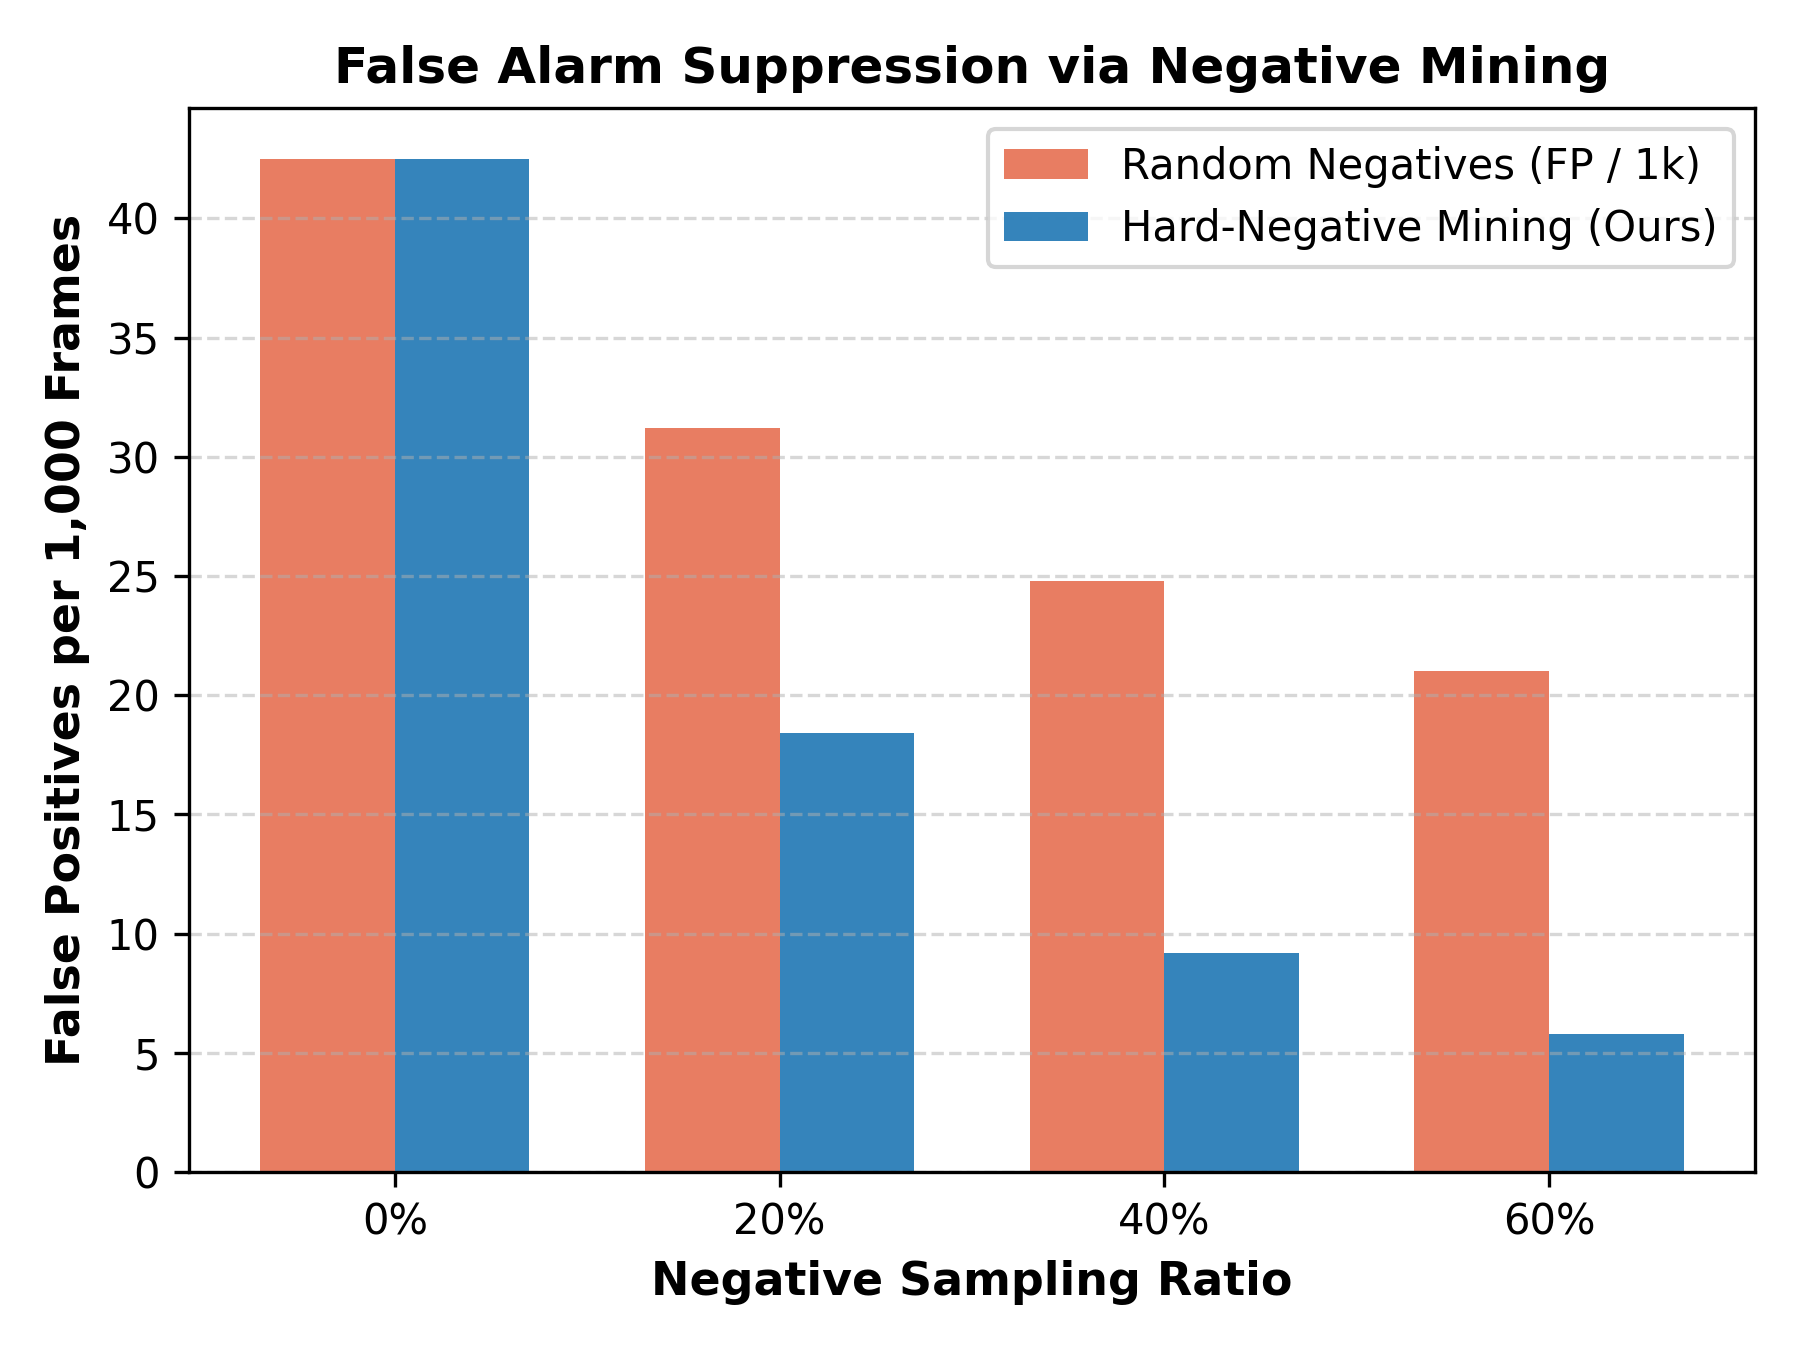
\includegraphics[width=\linewidth]{Figures/negativemining.png}
    \caption{Hard-negative mining}
    \label{fig:negative_mining}
  \end{subfigure}\hfill
  \begin{subfigure}[t]{0.48\linewidth}
    \centering
    % Verify whether 'roi.png' should be 'Figures/roi.png'
    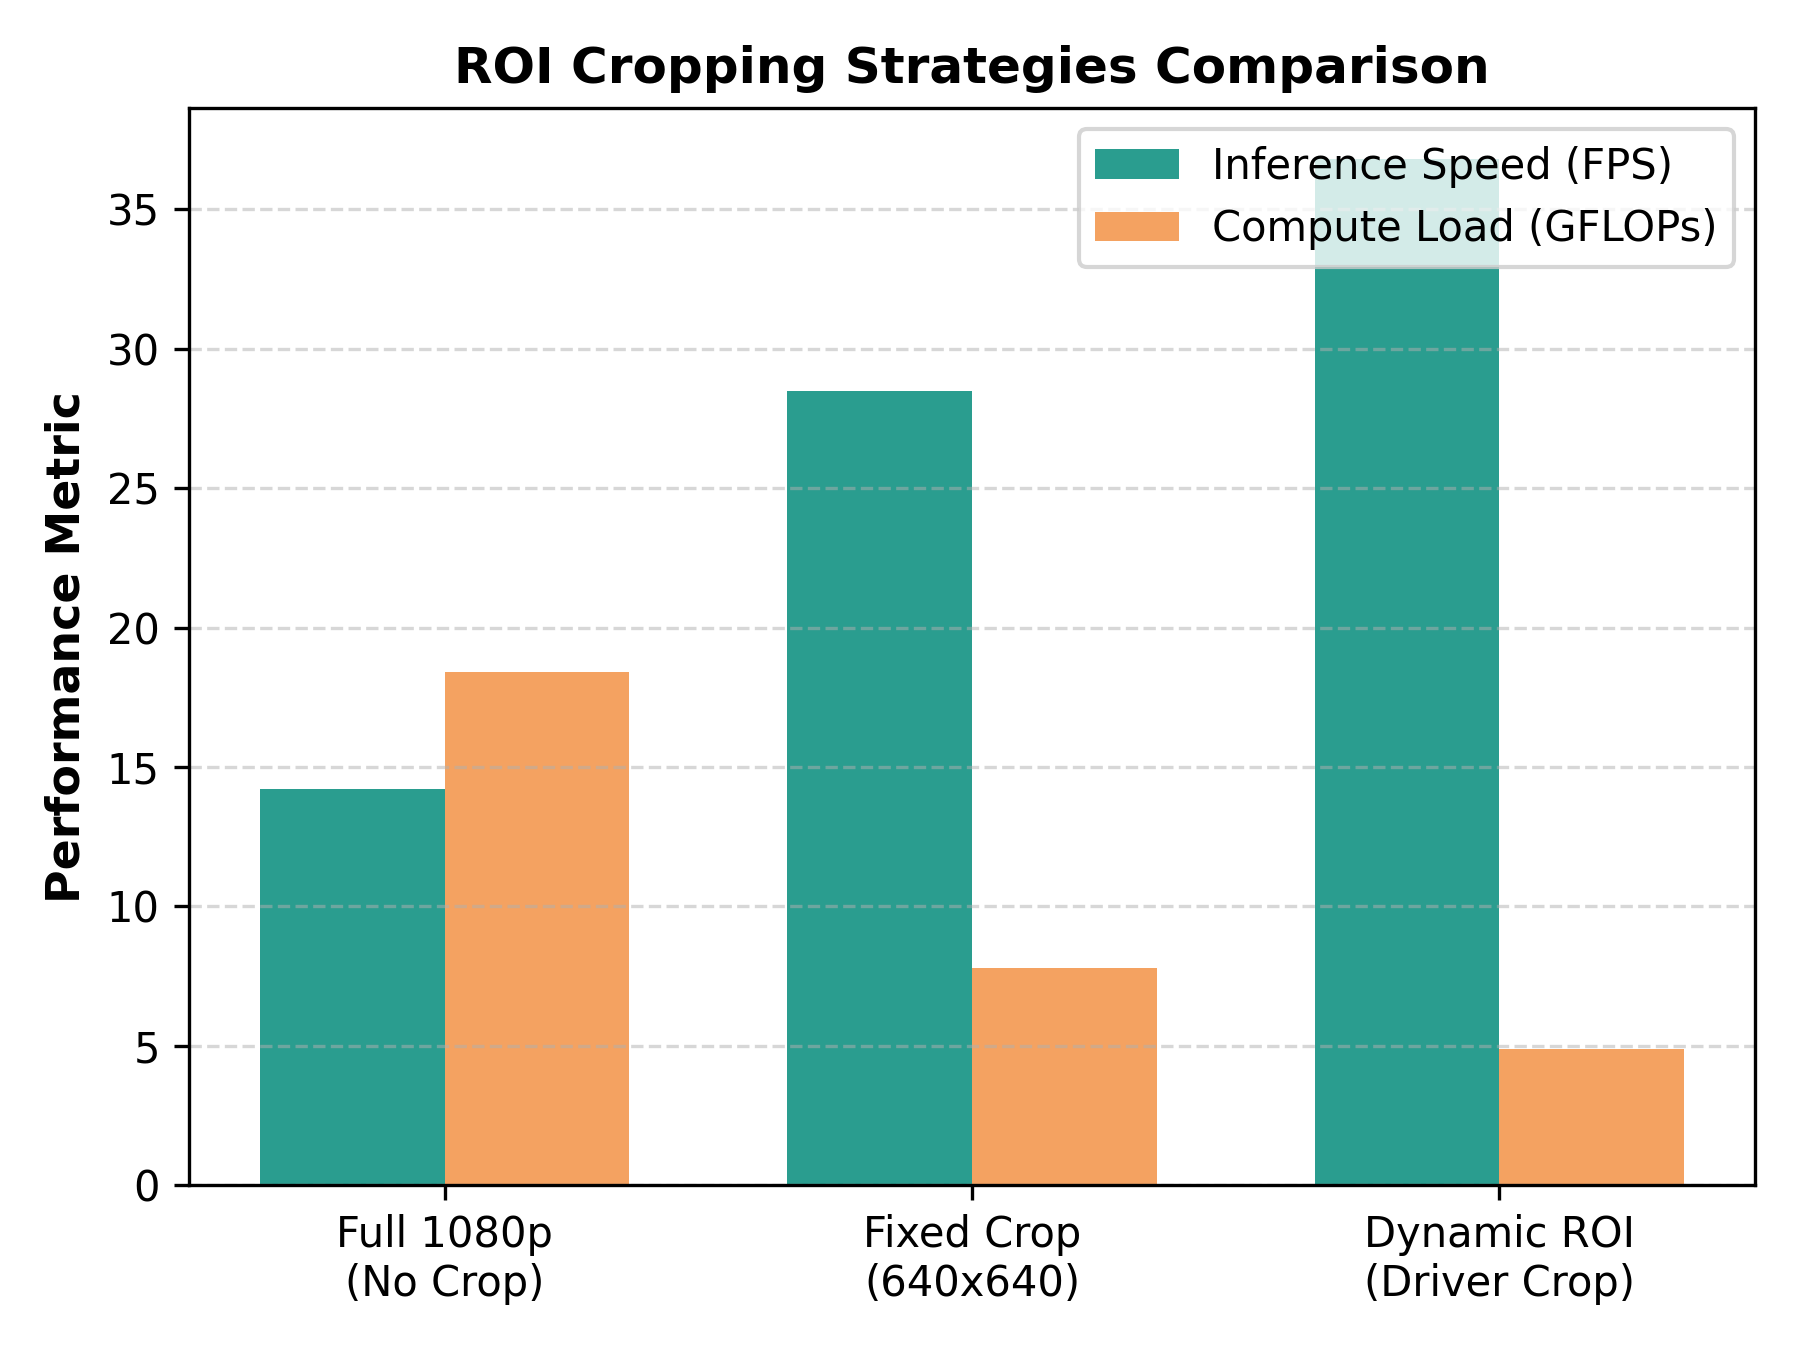
\includegraphics[width=\linewidth]{Figures/roi.png}
    \caption{\glsentryshort{roi} cropping methods}
    \label{fig:roi_cropping}
  \end{subfigure}
  \vspace{4pt}
  \caption[Empirical evaluation of hard-negative mining and ROI cropping strategies]{Empirical evaluation conducted in this work (\textbf{Ours}): \\(a) Suppression via hard-negatives ; and (b) Evaluating \glsentryshort{roi} cropping strategies.}
  \label{fig:empirical_studies}
\end{figure}

\subsection{Target Users and Markets}

We aim to provide this trustworthy solution to everyone. Primarily, our solution serves both the general public and commercial vehicle fleet operators. Specifically, government agencies such as Dubai's \gls{rta}, which deploys thousands of vehicles and employs personnel who drive for extended periods (such as taxi drivers), would benefit from a private, dependable safety system to support these operators.

\section{Scope and Feature Priorities}

Features are grouped by priority, "Required" features that deliver the base build, "Desired" features that will be delivered depending on the remaining time budget, and "Future" features that are out of scope of our \gls{sdp} 2. In the following sections we list the breakdown in detail.

\begin{table}[htbp]
\centering
\caption{Required System Feature Specifications}
\label{tab:req-features}
\footnotesize
\setlength{\tabcolsep}{4pt}
\renewcommand{\arraystretch}{1.15}
\begin{tabular}{|p{0.12\linewidth}|p{0.28\linewidth}|p{0.54\linewidth}|}
\hline
\textbf{Status} & \textbf{Title} & \textbf{Description} \\
\hline
Required & Deployment on Raspberry Pi 5 & The full detection pipeline runs live on the Pi 5. \\
\hline
Required & 1080p 30 \gls{fps} \gls{rgb} camera & A \gls{usb} 3.0 webcam aimed at the driver's face records 1080p at 30 \gls{fps}. Each frame is cropped to a fixed region before detection. \\
\hline
Required & Object detection model & \gls{yolo}11n detects drowsy and distraction classes. It is fine-tuned on the subject-disjoint dataset below. \\
\hline
Required & Temporal filtering (\gls{ema}) & An exponential moving average over each class score suppresses random single-frame spikes. It is defined in seconds, not frames, so it behaves the same at any FPS. \\
\hline
Required & Speaker and \gls{led} bar alert & After a confirmed detection, a bright \gls{led} bar flashes and a \gls{usb} 3.0 speaker plays a voice warning. \\
\hline
Required & Alert cool-down & Cheap and effective suppression for repeated warnings for the same event within a time frame.\\
\hline
Required & Mirror-check suppression & The classes (by design) do not depend on head orientation, so normal mirror checks and head turns do not trigger alerts. \\
\hline
Required & Internal logging & Each confirmed detection (time, type, confidence) is saved to the Pi's local storage. No raw video is kept by default. \\
\hline
Required & On-device video processing & All video processing happens on the Pi and raw video never leaves the vehicle. \\
\hline
Required & Subject-disjoint dataset collection & 10-minute \gls{rgb} in-cabin videos over several sessions, recorded in the morning and evening. Subjects are split so no subject appears in more than one of train, val, and test.\\
\hline
\end{tabular}
\end{table}

\begin{table}[htbp]
\centering
\caption{Desired System Feature Specifications}
\label{tab:desired-features}
\footnotesize
\setlength{\tabcolsep}{4pt}
\renewcommand{\arraystretch}{1.15}
\begin{tabular}{|p{0.11\linewidth}|p{0.27\linewidth}|p{0.56\linewidth}|}
\hline
\textbf{Status} & \textbf{Title} & \textbf{Description} \\
\hline
Desired & Model pruning and quantization & Pruning removes channels to cut \glspl{flop}. Quantization methods are compared on the Pi, choosing the best FPS while retaining detection metrics. \\
\hline
Desired & Hard-negative dataset & Subjects are re-recorded performing look-alike non-violations flagged by the baseline model. Only negative frames are added. \\
\hline
Desired & Neutral baseline clips & Each subject records a 20\,s neutral baseline clip to benchmark and evaluate calibration. \\
\hline
Desired & Class-specific alerting & Distinct alert tiers and voice notifications per class. \\
\hline
Desired & Tiered alert escalation & Gentle notification $\rightarrow$ voice prompt $\rightarrow$ multi-modal alarm (\gls{led} bar and voice) as risk persists. \\
\hline
Desired & Clear, explainable alerts & Contextual alerts (e.g., ``yawning detected 3 times in the last 5 minutes'') rather than generic warnings to build driver trust. \\
\hline
Desired & Camera-blind check & Measures frame brightness and sharpness. Logs and issues ``camera blocked'' warning if unclear for $\ge 3$\,s.\\
\hline
Desired & Driver-centered crop tracking & Lightweight face detector runs at $\sim 1$\,Hz on lower resolution frames to dynamically adjust the face crop. \\
\hline
Desired & New-driver calibration & Driver sits neutrally for 20\,s while detector runs at low confidence. Cutoffs set to 99th percentile $+$ a safe gap. Increasing the confidence threshold and reducing false alarms \\
\hline
Desired & Eye closure and micro-sleep alert & Face landmark tracking calculates \gls{ear}. Continuous closure triggers loud alert; 60\,s \gls{perclos} triggers gentle fatigue prompt.\\
\hline
Desired & Power-cut-safe logging & Database operates in \gls{wal} mode to prevent corruption during power interruptions. \\
\hline
Desired & Dashboard and cloud sync & Post-trip event records uploaded over \gls{tls} to update database and web dashboard with trends and metrics. \\
\hline
Desired & Actionable post-trip tips & Recommendations generated from logged behaviors (e.g., ``take a 30 minute break'')\\
\hline
Desired & Driver-facing tablet & Dedicated low-distraction glance-able \gls{ui}, allows for easy system calibration.\\
\hline
Desired & Pre-trip readiness check & Pre-drive fatigue survey on tablet recommending rest and nearby rest locations if fatigue is reported.\\
\hline
Desired & Rest-stop suggestions \gls{gps} & Queries \gls{gps} and \gls{poi} map services to recommend nearby rest stops or fuel stations when violations exceed a threshold. \\
\hline
\end{tabular}
\end{table}

\begin{table}[htbp]
\centering
\caption{Future System Feature Specifications}
\label{tab:future-features}
\footnotesize
\setlength{\tabcolsep}{4pt}
\renewcommand{\arraystretch}{1.15}
\begin{tabular}{|p{0.09\linewidth}|p{0.29\linewidth}|p{0.58\linewidth}|}
\hline
\textbf{Status} & \textbf{Title} & \textbf{Description} \\
\hline
Future & Driving-context suppression & Suppress or defer warnings during reversing maneuvers, standstill red lights, or high-density traffic.\\
\hline
Future & Multi-modal fusion & Aggregate multi-spectral video streams. \\
\hline
Future & Multiple camera feed & Additional camera to capture wide-angle context or secondary angles. \\
\hline
Future & Smartwatch and wearables integration & Incorporate driver heart-rate or biometric motion telemetry to augment edge detection.\\
\hline
Future & Robustness study & Systematic stress testing across glare, low light, optical blur, pose deviations, eyewear (glasses/sunglasses), face coverings, day-to-night transfer, and multi-vehicle cabins. \\
\hline
Future & Adaptive sensitivity by context & Context-aware threshold modification depending on the driver's behavior patterns. \\
\hline
Future & Steering wheel vibration & Haptic vibration on the steering wheel to reduce driver reaction latency.  \\
\hline
Future & Cabin comfort integration & System can change the \gls{ac} or change the volume of what's playing via the car's speakers. \\
\hline
Future & Voice recognition & Driver audio-interface enabling inquiries (e.g., ``How tired am I?''). \\
\hline
\end{tabular}
\end{table}
\newpage

\section{Proposal Overview and Revisions}

Our initial proposal covered the pre-development in detail, discussing a methodology for evaluating different object detectors and studying the effect of hard-negative mining. The primary focus was edge system performance on accuracy metrics and \glspl{fp} per 1000 frames. Since then, we changed the deployment hardware, upgrading from a Raspberry Pi 4 to a Pi 5 to provide better throughput and handle larger systems. We then pivoted the project to provide better \gls{ux} through various adaptive alerting mechanisms, nuisance filters, and system components such as web analytics or a user-friendly tablet interface.

\section{Project Roadmap}

We studied and evaluated different object detectors on \gls{rgb} and \gls{ir} public \gls{dms} datasets. Followed by evaluating negative-mining on false detections, and an empirical study on the trade-offs between temporal filters. Finally, we studied the effect of pruning, \gls{roi} cropping and input resolutions on performance. 

We will establish our organic in-cabin video dataset, with an extension of harder non-violation clips that will harden our detection model. Delivering a public subject-disjoint dataset. 

Before deployment, we perform an extensive literature review, to find what do drivers suffer from by using traditional \gls{dms}. Aiming to effectively counter these pain-points through careful system planning and design. we plan to document every design change meticulously. If the system faces technical complexity issues, we plan to surgically remove any non-required component, ensuring project delivery on time.

Post-deployment, we evaluate the system by involving users for their feedback, adequate testing and taking recommendations from peers, allowing the project to develop and adapt to fit the end user the best.

\section{Report Organization}

To end this chapter, here is a breakdown on how this report is organized:

In Chapter II, we explore current limitations and shortcomings in existing \gls{dms} work, providing a gap summary highlighting the need for better \gls{ux} in said systems.

In Chapter III, we deep-dive into the technical concepts and principles of deploying complex \glspl{dms}.

In Chapter IV, we report in detail our proposed solution, funneling a general idea into a detailed look at every component in the system. To provide a complete report, project constraints and issues are discussed.

Chapter V includes the methodology, highlighting the empirical methods we used to evaluate, organize and build the system and its dataset.

Finally Chapter VI summarizes the main findings, lists the project milestones and discusses what we aim to work on in \gls{sdp} 2.


\chapter{Literature Review}
This chapter explores the rapid growth in the utilization of \glspl{uav} and the associated risks, particularly as UAVs become increasingly integrated into civil, commercial, and defense sectors. Their transformative impact on air operations is largely attributed to advancements in navigation, sensing technologies, and miniature satellites. Today, \glspl{uav} are deployed in diverse applications such as agriculture, logistics, environmental monitoring, and infrastructure inspection. However, despite their capabilities, \glspl{uav} pose significant challenges, particularly in airspace management—specifically regarding collision avoidance, traffic coordination, and adherence to no fly zones.



\chapter{Technical Background}
\input{Chapters/Chapter_3}

\chapter{Proposed Solution}
\input{Chapters/Chapter_4}

\chapter{Research Methodology}
\input{Chapters/Chapter_5}

\bibliographystyle{plainnat}
\bibliography{Bibliography/references}

\end{document}
